The broad purpose of the FieldConvert utility is to read in data from a file, perform some operation on this data, and write the data resulting from this operation to an output file. To illustrate how it does this, let us consider a case in which the user wishes to calculate the wall shear stress on the boundary labelled \verb+"0"+, given a session file \verb+session.xml+ and field file \verb+field.fld+, and write it to field file \verb+field_wss.fld+ at $10$ equispaced points using the \inltt{output-points} option  \footnote{The output file would actually be \texttt{field\_wss\_b0.fld}.}

\begin{lstlisting}[style=BashInputStyle]
FieldConvert -n 10 -m wss:bnd=0 session.xml field.fld field_wss.fld
\end{lstlisting}

The first task is to determine how to proceed based on the user input on the command line. In this case, each command line input apart from \inltt{-n 10} corresponds to a module. The program stores these inputs as a  \verb+boost::program_options::variables_map+ object, in which each input is the key and its corresponding argument (if it has one) is the value. The key is a \verb+std::string+, and the value is optional, and can be any type. 

The names of process modules are specified using the flag\inltt{-{}-module} or \inltt{-m}, and these are stored in the map using the key \verb+"module"+ and the value being whatever follows the flag, in this case the \verb+"wss:bnd=0"+. The file names, corresponding to input and output modules, are so-called \textit{hidden options}, meaning they don't require a flag. These are stored in the map using the key \verb+"input-file"+, with the value being a \verb+std::vector+ consisting of the filenames, in this case \verb+"session.xml"+, \verb+"field.fld"+, and \verb+"field_wss.fld"+. The \inltt{output-points} option is stored in the map using the key \verb"output-points" and the value being \verb+10+.


Assuming the user did not specify the command line options \inltt{help}, \inltt{modules-list}, or \inltt{modules-opt}, the program proceeds with its main functionality and a \verb+FieldSharedPtr+ is constructed. The values in the map corresponding with the \verb+module+ and \verb+input-file+ keys are stored as a \verb+std::vector+ of \verb+std::string+s called the \textit{module commands}, with the values corresponding to input modules at the start, process modules in the middle, and output modules at the end. Note that the program assumes that all these files apart from the last are input files, unless specified by the prefix \inltt{out} on the command line:, e.g. \inltt{out:file.fld}.


The module commands are iterated over, and for each entry, the the module string is identified and stored with the module type in a \verb+ModuleKey+. For input modules, the module string is identified using \verb+InputModule::GuessFormat()+, or failing that, by taking the name of the file extension, as is done for output modules. For process modules, the module string is simply the name of the entry (up to the colon separator if there is one). The \verb+ModuleKey+ is used to create a \verb+ModuleSharedPtr+ using the factory by calling \verb+Module::GetModuleFactory().CreateInstance+, passing the \verb+ModuleKey+ and the \verb+FieldSharedPtr+ as arguments. This \verb+ModuleSharedPtr+ is appended to a \verb+std::vector+ of \verb+ModuleSharedPtr+s. For input modules, \verb+InputModule::AddFile+ is called with the module string and the input file name passed as arguments. The configuration options are then parsed and registered using \verb+Module::RegisterConfig()+, with arguments being the option name and its value (if it is boolean, the argument is just the option name). For input and output modules, the option \verb+infile+ or \verb+outfile+ is passed, along with the input or output file name. To complete the loop, the \verb+Module::SetDefaults+ function is called. The process of constructing a module, registering the configuration options (as well as calling \verb+AddFile+ for \verb+InputModule+s), and setting the default configuration options for those that were not set is summarised as \textit{setting up} the module. The processes involved in the set up of input, process, and output modules are shown in figure \ref{fig:setupmodule}. In this case, instances of the \verb+InputXml+, \verb+InputFld+, \verb+ProcessWSS+, and \verb+OutputFld+ classes are constructed. The configuration option name for \verb+InputXml+ and \verb+InputFld+ is the string \verb+infile+ and the values are the filenames \verb+session.xml+ and \verb+field.fld+ respectively. The option for \verb+ProcessWSS+ is \verb+bnd+ with value \verb+0+, and the option name for \verb+OutputFld+ is the string \verb+outfile+ with the value being the filename \verb+field_wss.fld+. Then, a \verb+ModuleSharedPtr+ is created for the \verb+ProcessEquispacedOutput+ module if it is needed. \footnote{This module is needed for certain combinations of modules} The \verb+CheckModules+ function (defined \verb+FieldConvert.cpp+ is called with the \verb+std::vector+ of \verb+ModuleSharedPtr+s as argument in order to check the modules that have been set up are compatible. Finally, the \verb+RunModule+ function (defined in \inlsh{FieldConvert.cpp}) is called with each \verb+ModuleSharedPtr+ as argument in order of priority, which essentially calls the \verb+Process+ function as for each module, operating on the various member variables of \verb+Field+, with the map used to store the command line arguments passed to each. When using the \inltt{nparts} command line argument, the calling of \verb+RunModule+ is done in a loop over the number of partitions. On each iteration, \verb+Field::ClearField+ is called, and a new \verb+Comm+ object is generated called \verb+partComm+ using the current partition number, with the original saved as \verb+defComm+. \verb+Field+'s \verb+m_comm+ is switched to \verb+partComm+ when running \verb+InputXml+ or any output module, and kept as \verb+defComm+ otherwise.

%Running \verb+InputXml+ populates \verb+m_session+ and \verb+m_graph+ using \verb+session.xml+ stored in \verb+m_inputfiles+, and running \verb+InputFld+ populates \verb+m_fielddef+, \verb+m_graph+, \verb+m_data+, \verb+m_variables+, and \verb+m_fieldMetaDataMap+. The

%All these bar the last, as well as \verb+m_requireBndExp+ and \verb+m_declareExpansionAsContField+ are used when populating \verb+m_exp+ at the start of running \verb+ProcessWSS+. This module then updates \verb+m_exp+ to include an expansion for the wall shear stress. Finally, running \verb+OutputFileBase+ (the parent class of \verb+OutputFld+) writes the wall shear stress to file using \verb+m_exp+ and \verb+m_fieldMetaDataMap+. Both \verb+ProcessWSS+ use \verb+OutputFld+ make use of the fact that \inltt{output-points} was specified on the command line.
A diagram of the process is shown in figure \ref{fig:fieldconvert}. It shows the order in which the modules are set up and run, and what member variables of \verb+Field+ each updates. The key for the diagrams in this section is shown in figure \ref{fig:fieldconvertkey}.


\begin{figure}[htbp]
\centering
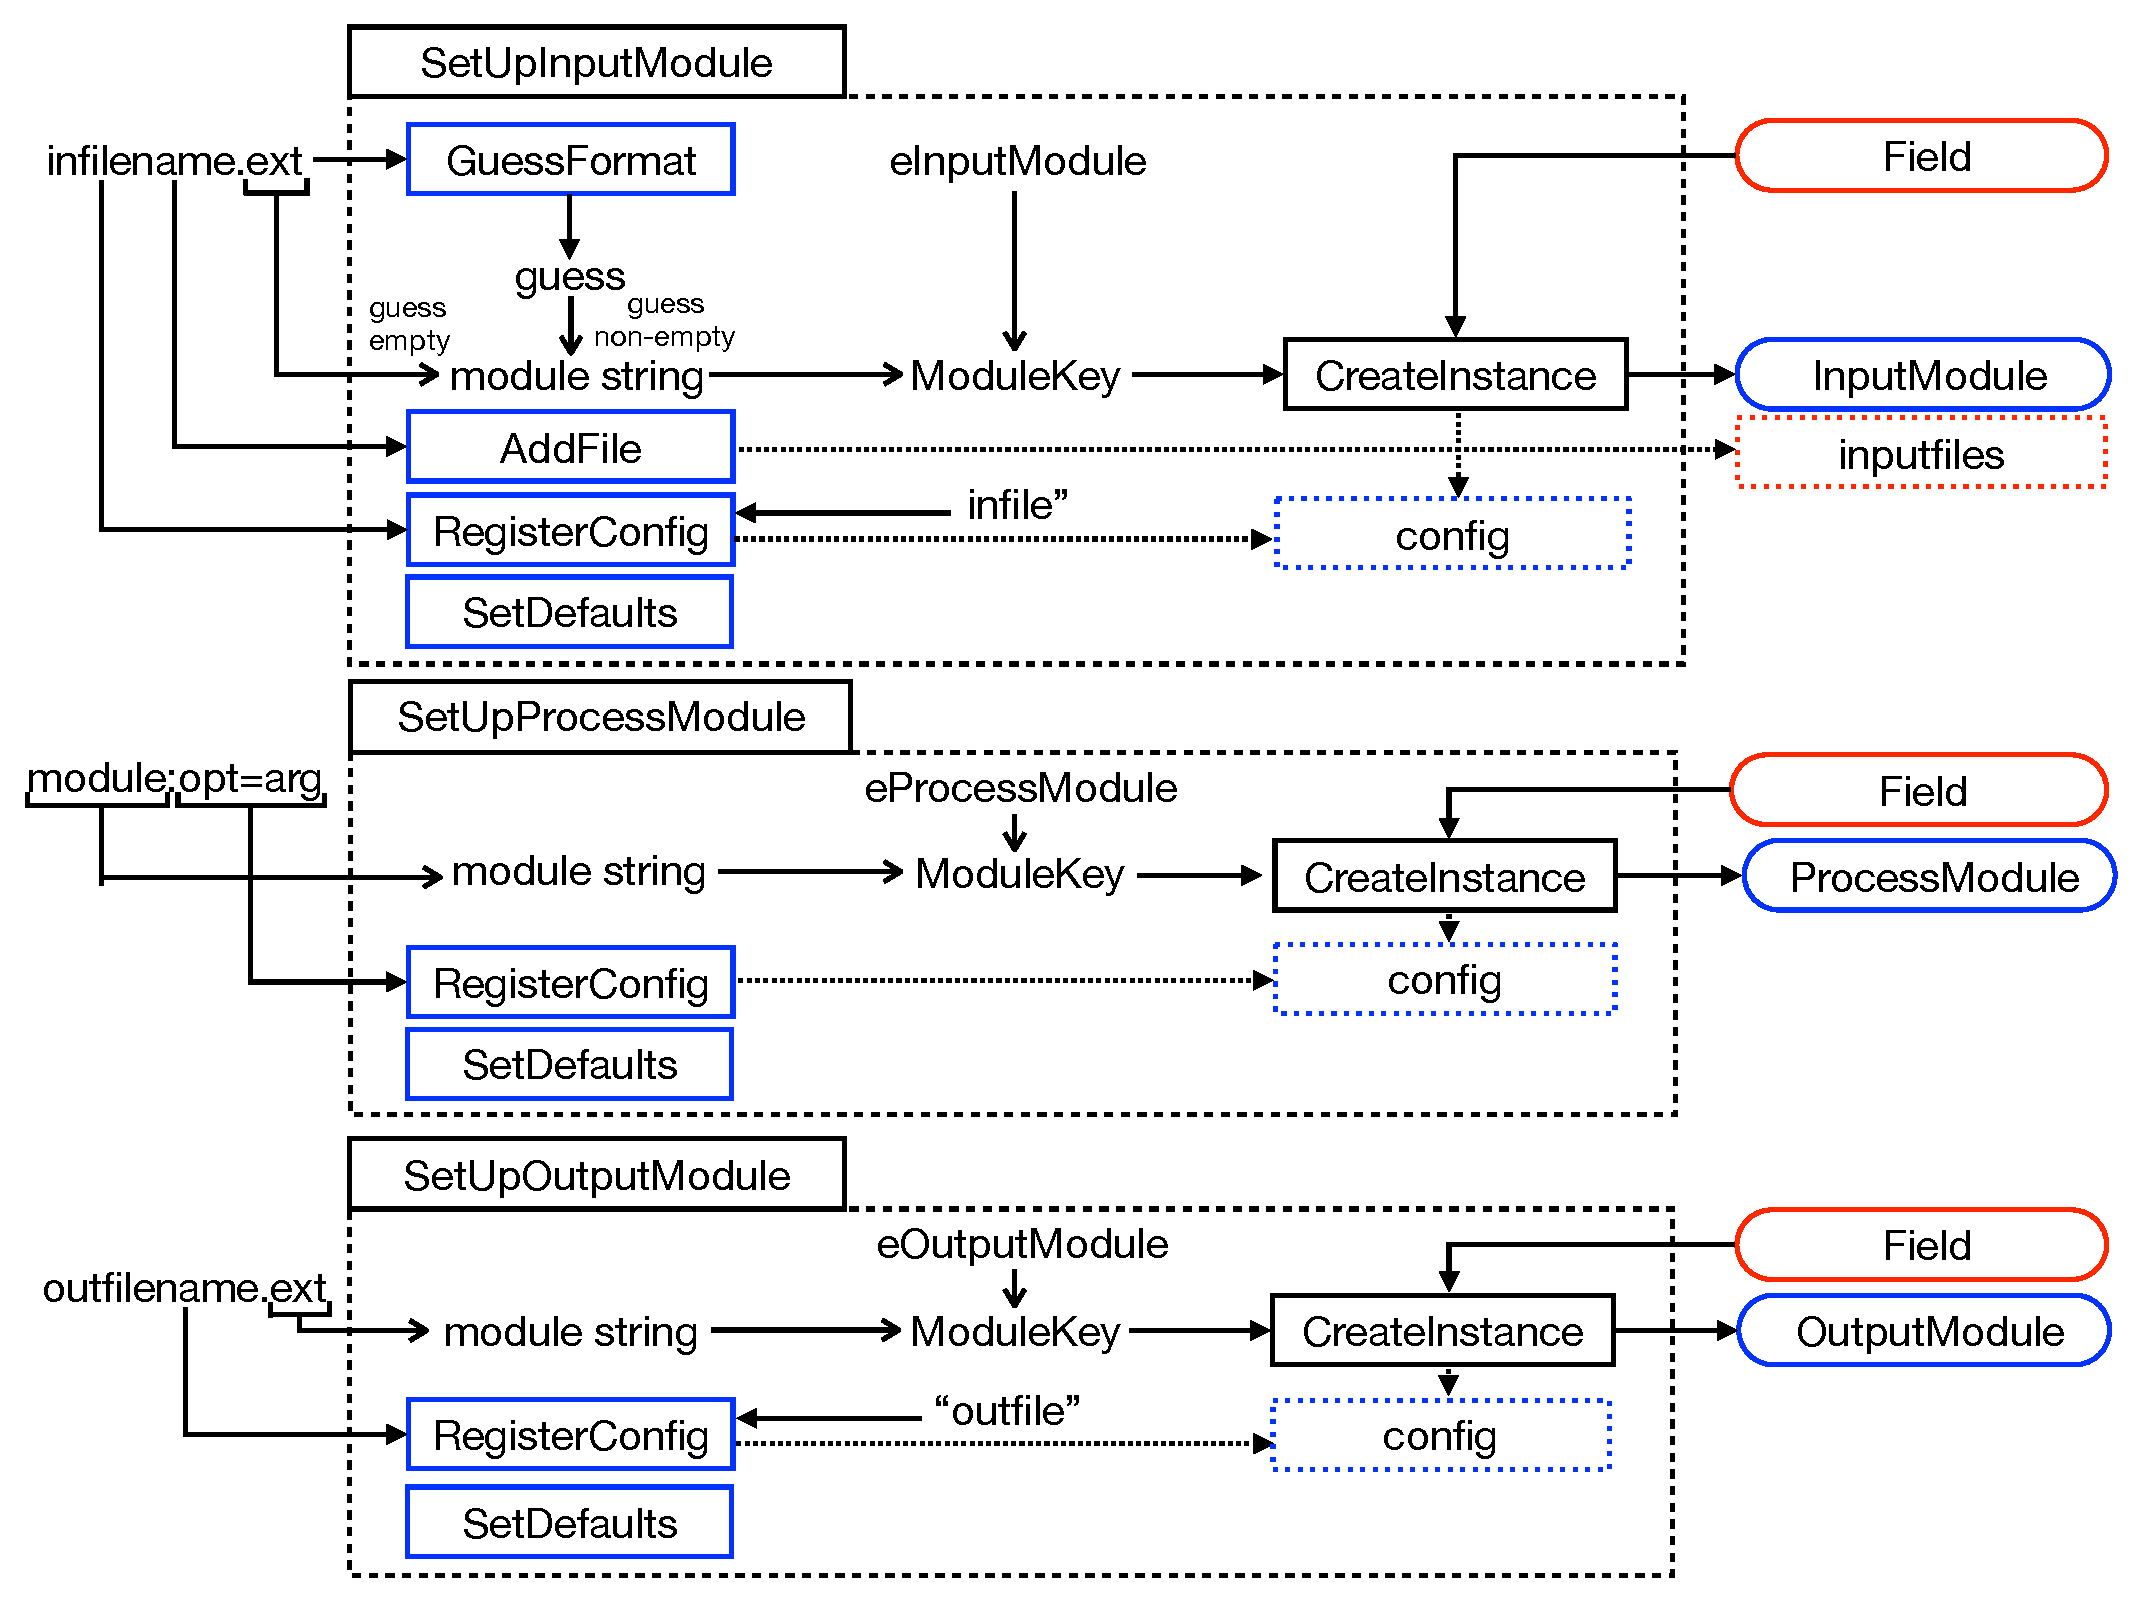
\includegraphics[width=\linewidth]{utilities/img/SetUpModule.pdf}
\label{fig:setupmodule}
\caption{Setting up modules} 
\end{figure}

\begin{figure}[htbp]
\centering
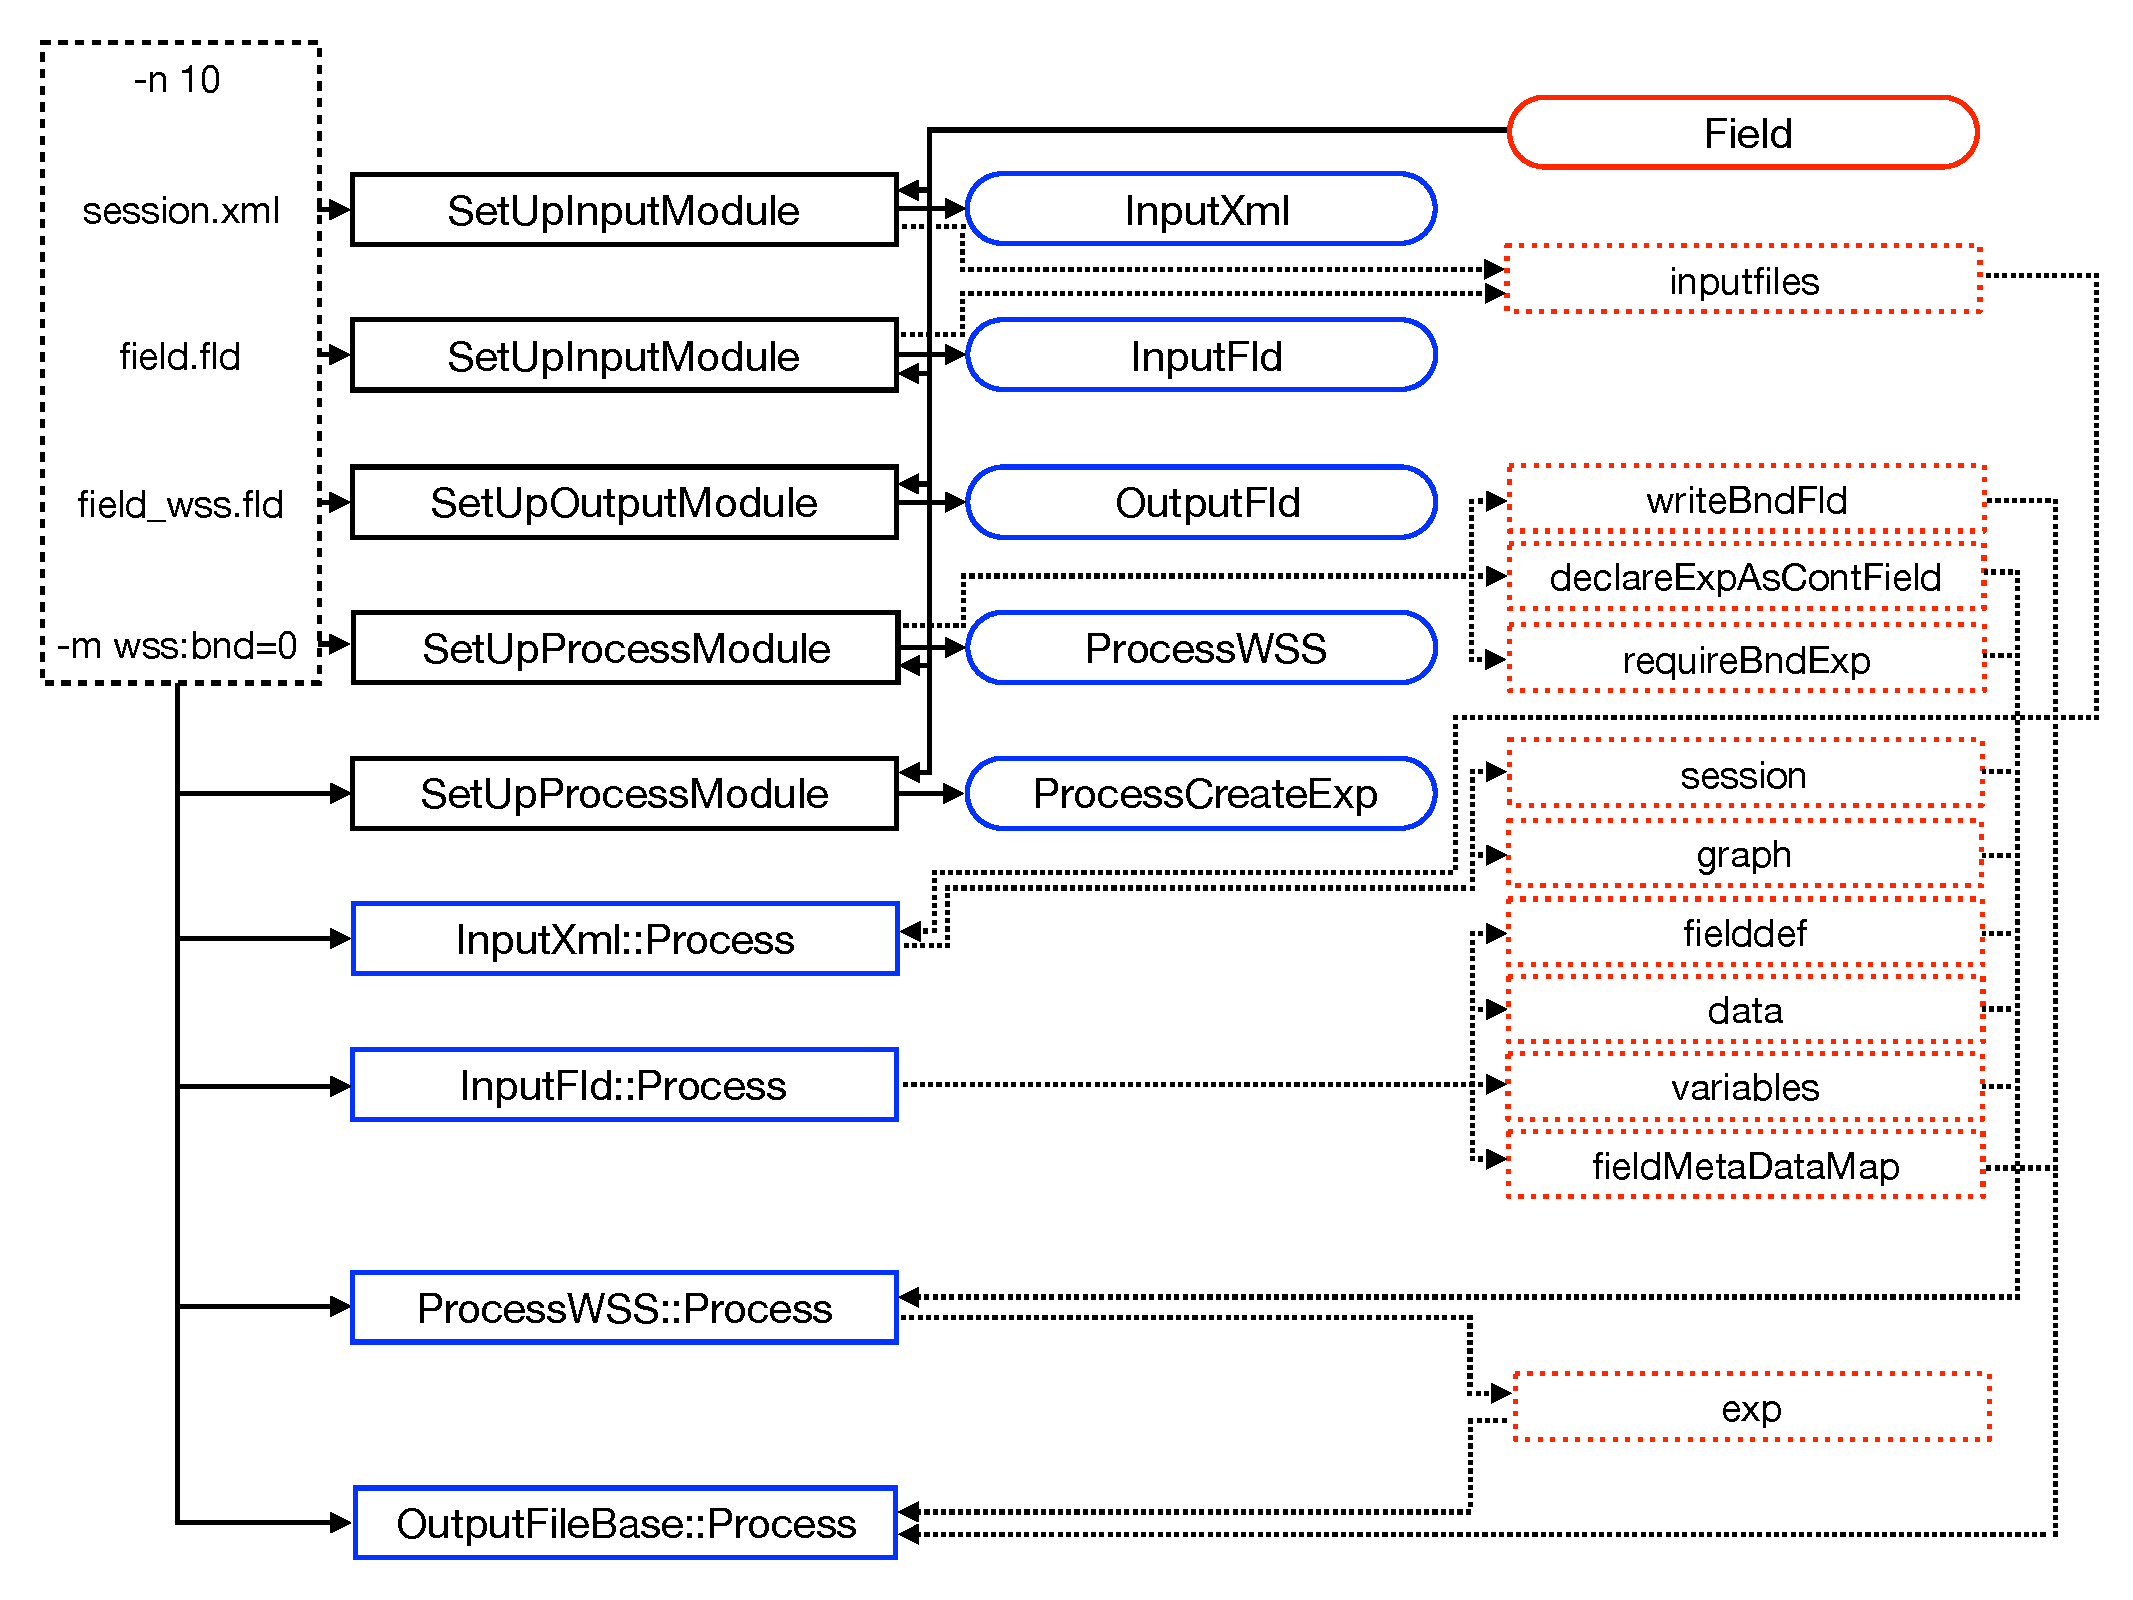
\includegraphics[width=\linewidth]{utilities/img/FieldConvertNew.pdf}
\label{fig:fieldconvert}
\caption{A diagram showing how FieldConvert performs a task} 
\end{figure}

\begin{figure}[htbp]
\centering
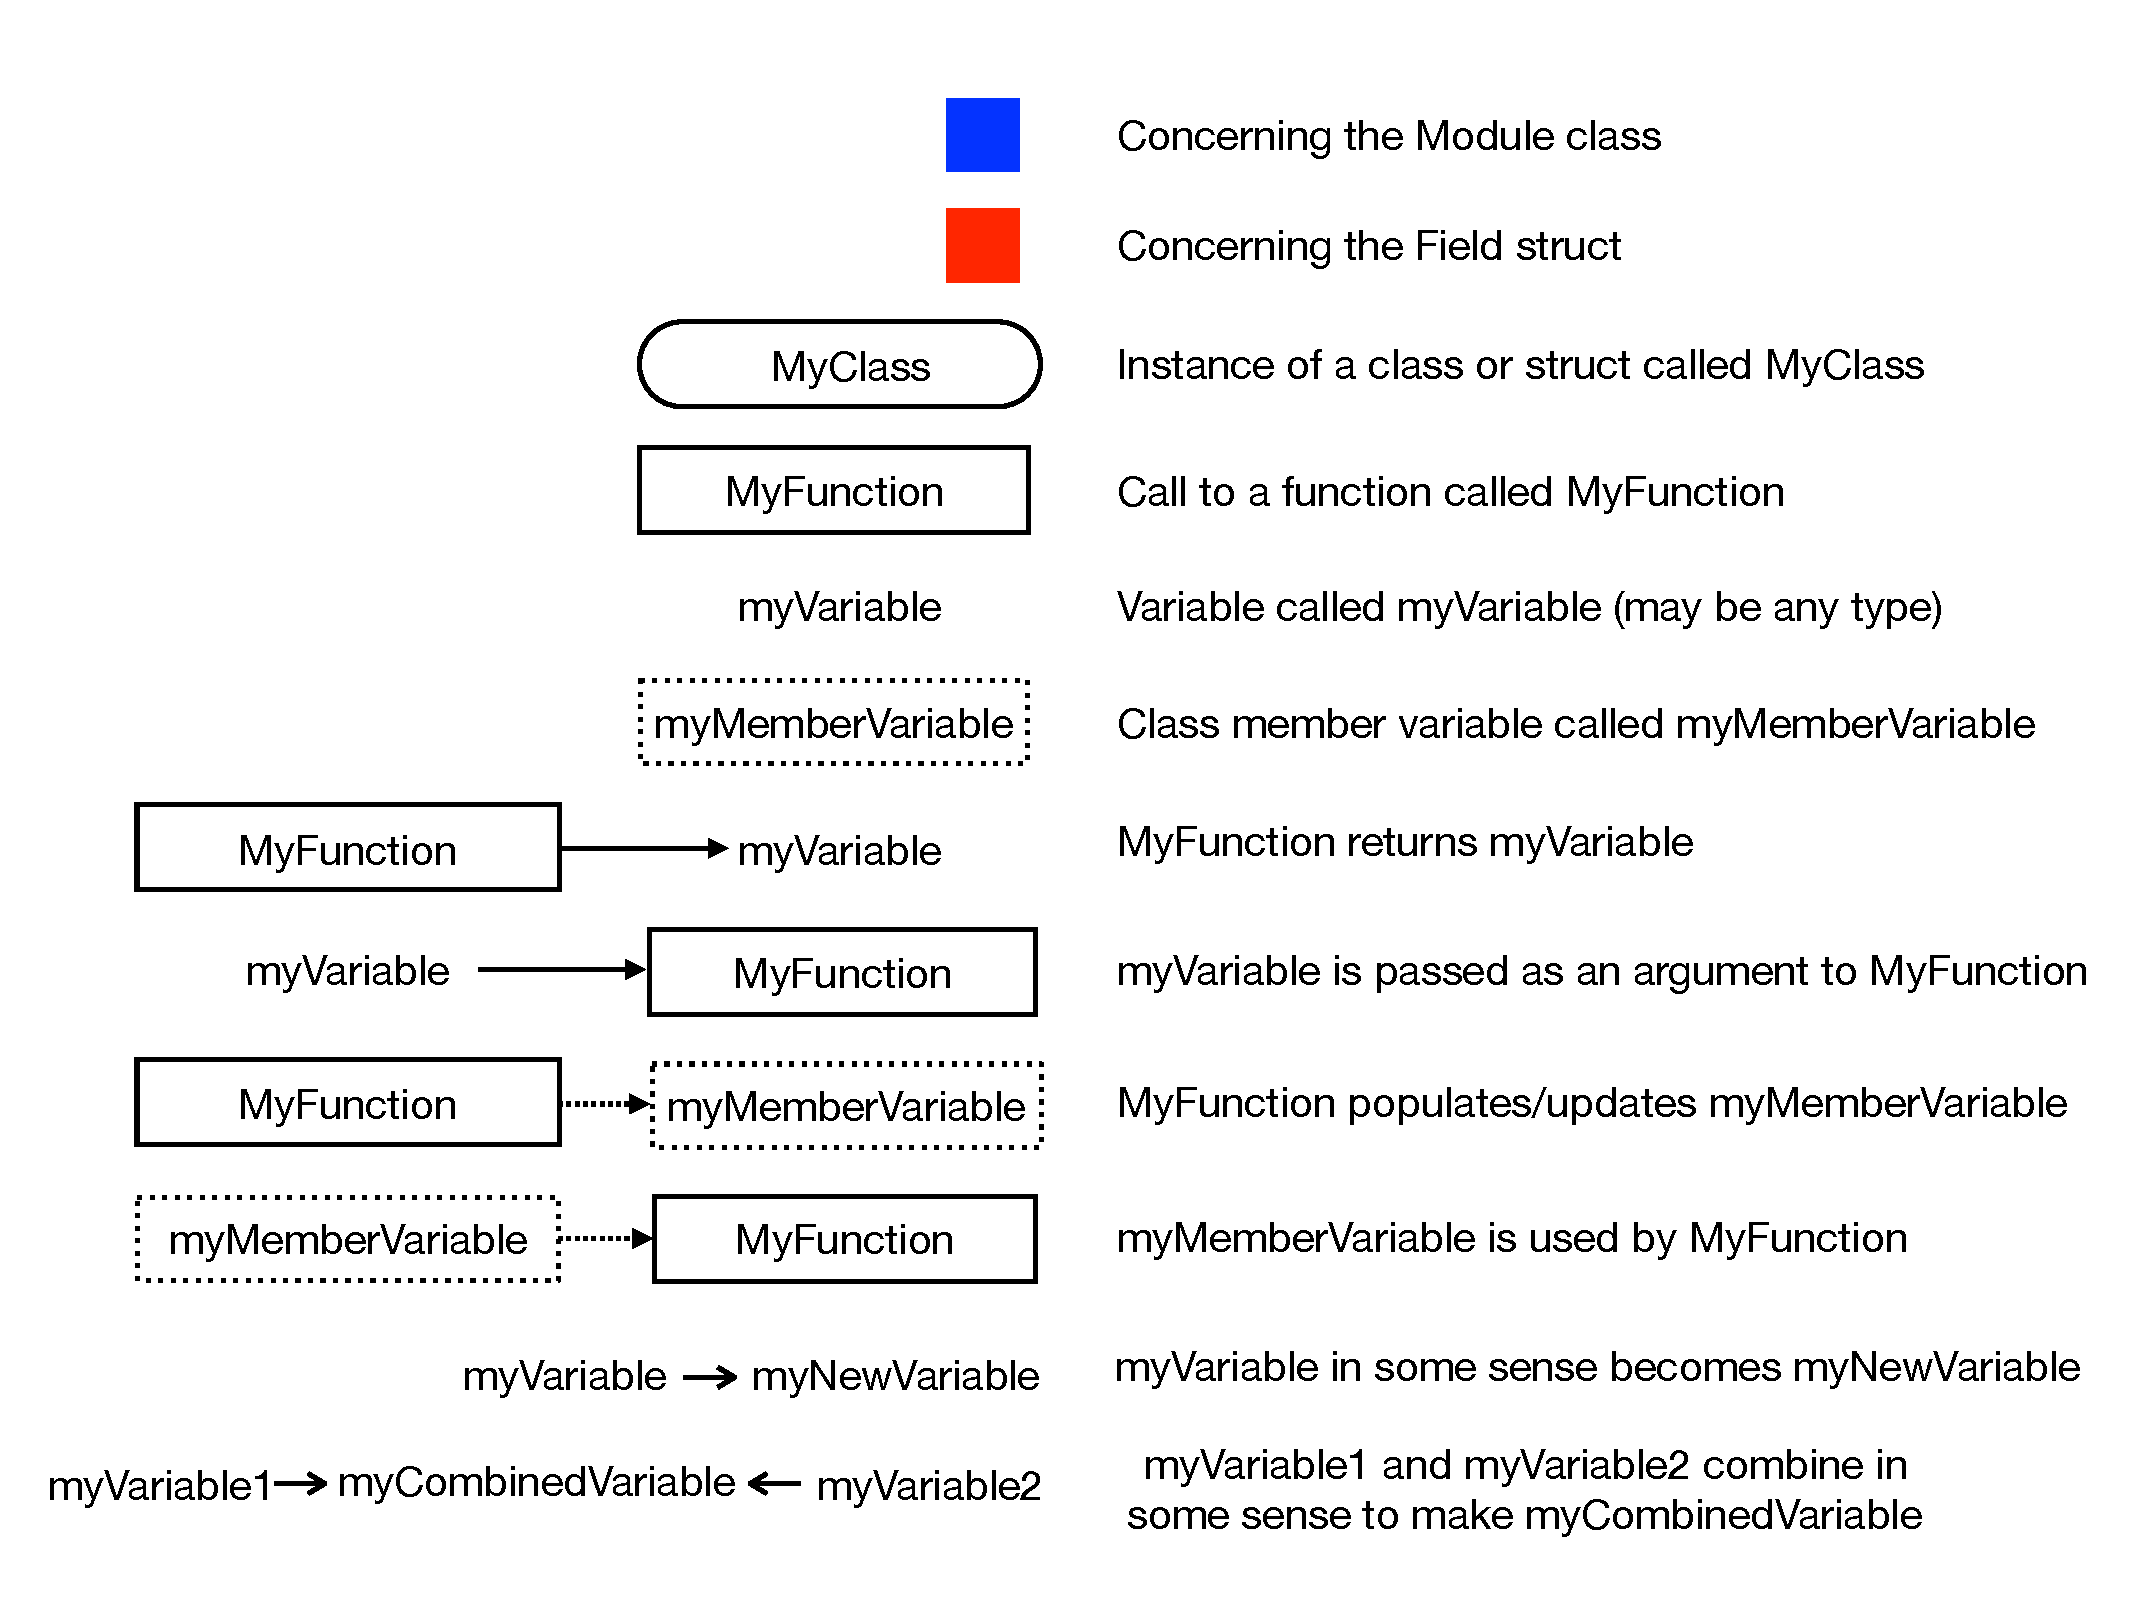
\includegraphics[width=\linewidth]{utilities/img/Key.pdf}
\label{fig:fieldconvertkey}
\caption{Key for the diagrams in this section} 
\end{figure}












